\documentclass{beamer}
\usepackage[english,russian]{babel}
\usepackage[utf8]{inputenc}
\usepackage{amsmath}
\usepackage{hyperref}
\usetheme{Warsaw}
\usepackage{listings}
\usepackage{xcolor}
\usepackage{tikz}
\usetikzlibrary{graphs}
\usepackage{algpseudocode}

\lstset{
    frame=tb,
    tabsize=4,
    showstringspaces=false,
    numbers=left,
    commentstyle=\color{green},
    keywordstyle=\color{blue},
    stringstyle=\color{red},
    emph={baz},
    emphstyle=\textbf
}

\begin{document}

\title{SAT/SMT solvers\newline  3. Davis–Putnam–Logemann–Loveland(Theory)}
\author{Roman Kholin}
\institute{Lomonosov Moscow State University}
\date{Moscow, 2023}

\begin{frame}
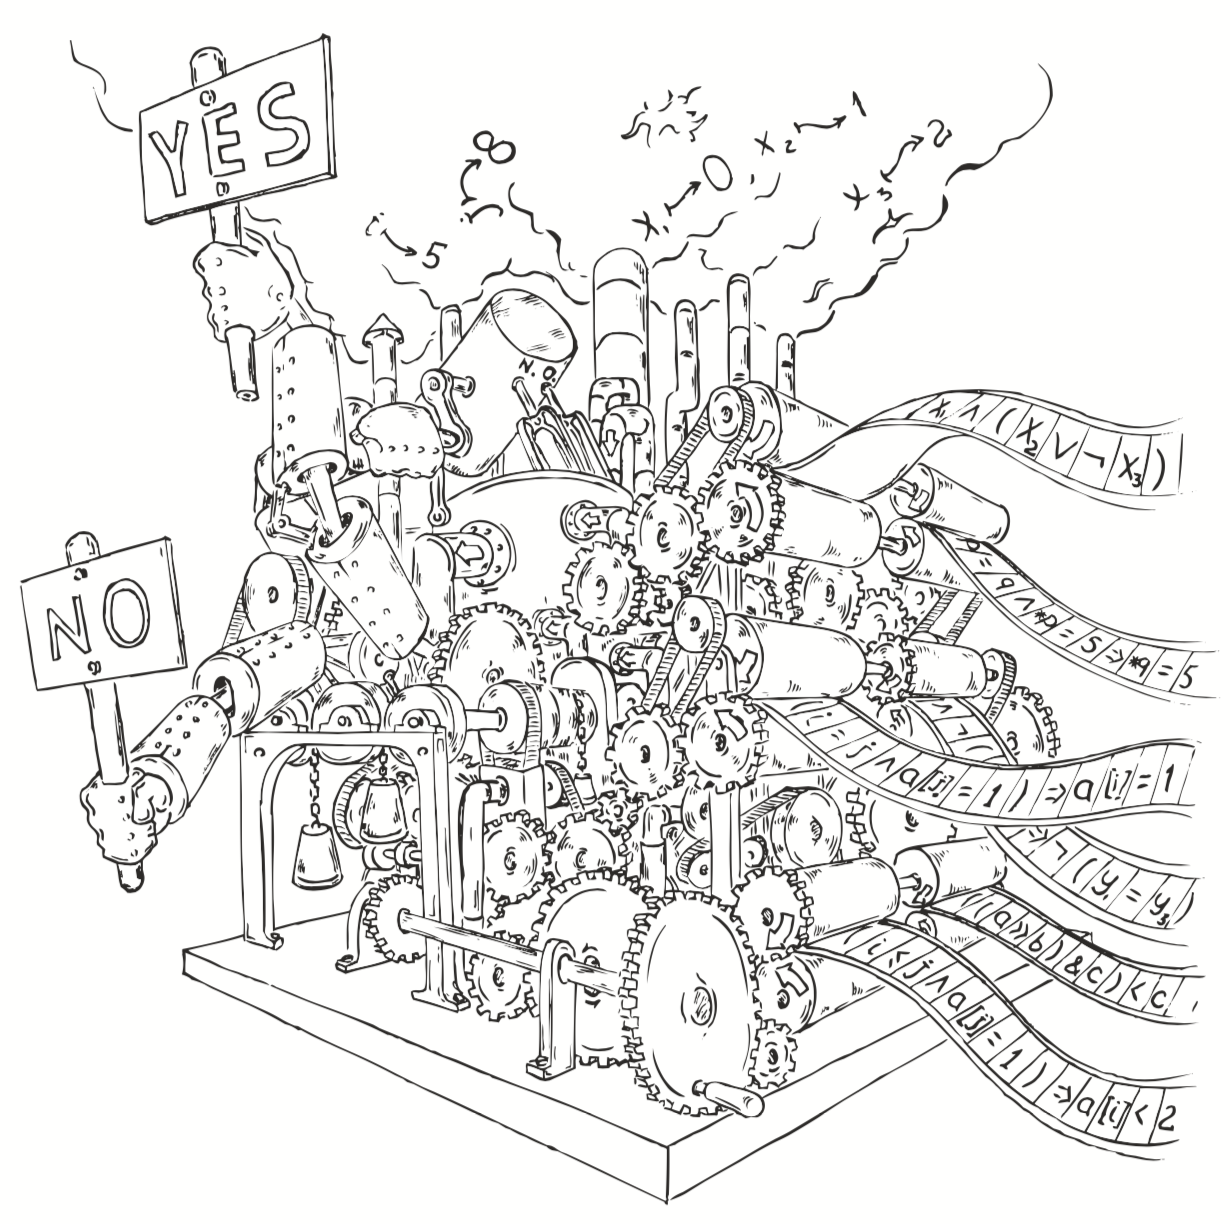
\includegraphics[scale=0.5]{../decision-procedure.png}
\end{frame}

\frame{\titlepage}

\begin{frame}{Definitions}
\begin{block}{}
\begin{itemize}
\item $at(\varphi)$ - the set of $\Sigma$-atoms in a given NNF formula $\varphi$
\item $at_i(\varphi)$ - the $i$-th distinct atom in $\varphi$
\item $e(\varphi)$ - Boolean variable called encoder of this atom
\item $e(\varphi)$ - Boolean formula resulting from substituting each $\Sigma$-atom in $\varphi$ with its Boolean encoder
\end{itemize}
$e(\varphi)$ is also called propositional skeleton of $\varphi$
\end{block}
\begin{itemize}
\item $\varphi := x = y \vee x = z$
\item $at_1(\varphi) := x = y, at_2(\varphi) := x = z$
\item $e(x = y) := b_1$
\item $e(x = z) := b_2$
\item $e(\varphi) := b_1 \vee b_2$
\end{itemize}
\end{frame}

\begin{frame}{Definitions}
\begin{block}{}
\begin{itemize}
\item $\alpha$ - assignment of $e(\phi)$
\item $Th(at_i, \alpha) = at_i$, if $\alpha(at_i) = TRUE$, $\lnot at_i$ otherwise
\item $Th(\alpha) = \{Th(at_i, \alpha)| для всех e(at_i), оцененных \alpha\}$
\item $\overline{Th(\alpha)}$ - conjunction of $Th(\alpha)$
\end{itemize}
\end{block}
$\varphi := x = y \wedge ((y = z \wedge \lnot(x = z)) \vee x = z)$
\end{frame}

\begin{frame}

\includegraphics[scale=0.45]{pineapple}
\end{frame}

\begin{frame}{Lazy SMT}
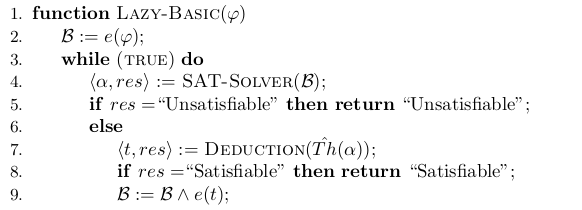
\includegraphics[scale=0.5]{Lazy_SMT1.png}
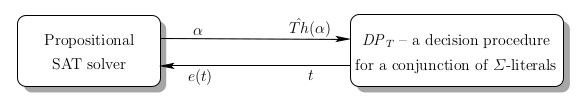
\includegraphics[scale=0.5]{Lazy_SMT.png}
\end{frame}

\begin{frame}{Lazy CDCL}
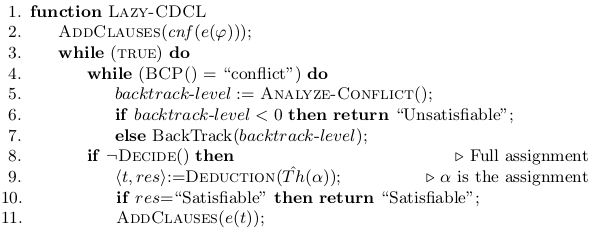
\includegraphics[scale=0.5]{Lazy_CDCL.png}
\end{frame}

\begin{frame}{DPLL(T)}
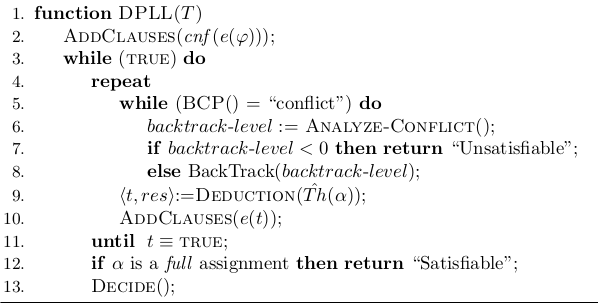
\includegraphics[scale=0.5]{DPLL1.png}
\end{frame}

\begin{frame}{DPLL(T)}
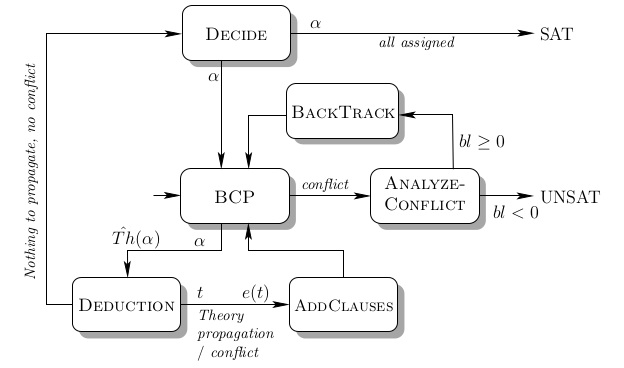
\includegraphics[scale=0.5]{DPLL2.png}
\end{frame}

\begin{frame}
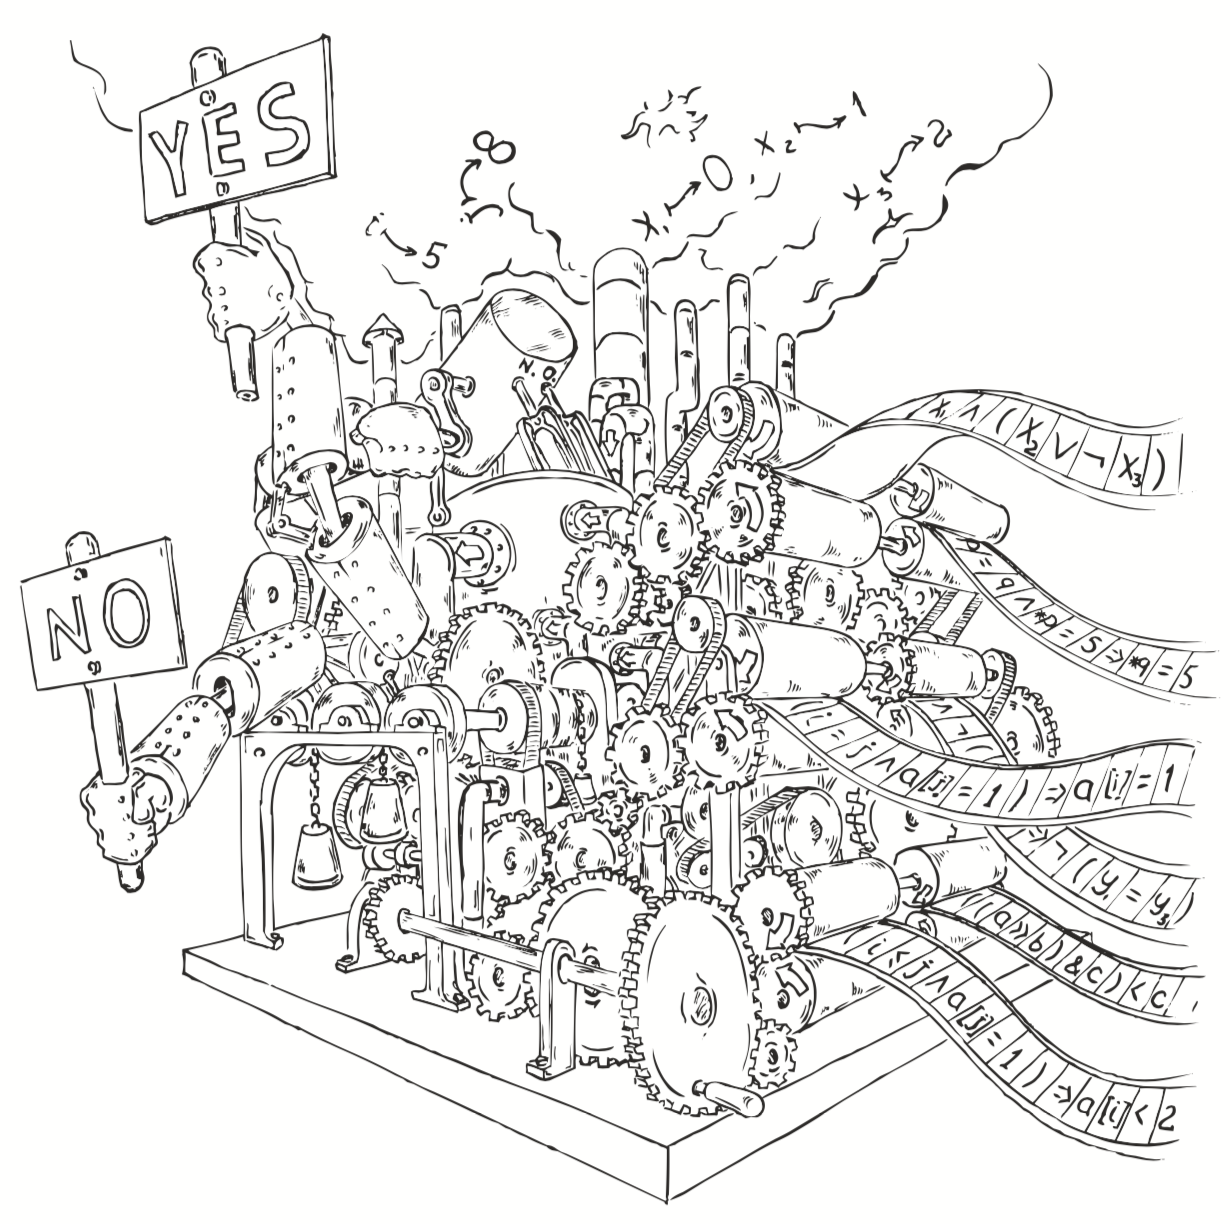
\includegraphics[scale=0.5]{../decision-procedure.png}
\end{frame}

\end{document}
